\documentclass[a4paper]{article}
\usepackage{titling}
\usepackage{authblk}
\usepackage{fancyhdr}
\usepackage{hyperref}
\usepackage{rsc}
\usepackage{siunitx}
\usepackage{graphicx}
\usepackage{listings}
\usepackage{color}

\definecolor{dkgreen}{rgb}{0,0.6,0}
\definecolor{gray}{rgb}{0.5,0.5,0.5}
\definecolor{mauve}{rgb}{0.58,0,0.82}

\lstset{frame=tb,
  language=Python,
  aboveskip=3mm,
  belowskip=3mm,
  showstringspaces=false,
  columns=flexible,
  basicstyle={\ttfamily},
  numbers=none,
  numberstyle=\tiny\color{gray},
  keywordstyle=\color{blue},
  commentstyle=\color{dkgreen},
  stringstyle=\color{mauve},
  breaklines=true,
  breakatwhitespace=true,
  tabsize=3
}


\title{Lecture 1: Introduction to Python}
\author[1]{Dr Benjamin J. Morgan}
\author[1,2]{Dr Andrew R. McCluskey}
\affil[1]{Department of Chemistry, University of Bath, email: b.j.morgan@bath.ac.uk}
\affil[2]{Diamond Light Source, email: andrew.mccluskey@diamond.ac.uk}
\setcounter{Maxaffil}{0}
\renewcommand\Affilfont{\itshape\small}

\pagestyle{fancy}
\fancyhf{}
\rhead{CH40208}
\lhead{\thetitle}

\begin{document}
\maketitle

\section*{Aim}
In this lecture, you will be introduced to Pythonic variable types, basic arithmetic, input and output (I/O) and intrinsic functions. 

\section{Introduction}

The aim of this course is to develop skills in the user of computer programming (particularly in the Python programming language), building on the skills learned in the first and second year Computational Chemistry laboratory. :w

You will then put these skills into practice, using Python to analyse chemical structures and perform quantum mechanical chemical calculations. 

The Python programming language is one of the most popular programming languages in the world, ranking third on the TIOBE index (a measure of programming language popularity) in June 2019\cite{tiobe_index}, with the largest rate of change. 
Additionally, it is probably the most popular programming language used in the chemical sciences. 
Recently, it was suggested that more than \SI{7}{\percent} of all academic papers published in 2018 made mention of the Python (Figure~\ref{fig:pic}) \cite{arm_pycon}. 
%
\begin{figure}[h]
\centering
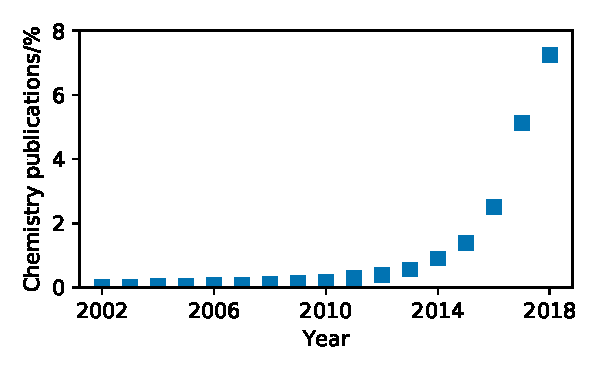
\includegraphics{chem_data_py}
\caption{The percentage of ``chemistry'' publications that also mention ``python'', determined from the numbers of matching Google Scholar results.}
\end{figure}
%

Python was first released in 1991, with one of the main design philosophies of the language being code readability. 
This readability is one of the driving factors to its adoption, along with some of the concepts introduced in this course, such as dynamical typing and powerful libraries like NumPy and Matplotlib. 
Since the early 1990s there have been three major versions of Python, with the most recent (and the focus of this course) being Python 3. 
Python 2 is still commonly found online and in libraries, however it is due to ``retire'' at the end of this year (check out \url{https://pythonclock.org} for a live countdown). 
Therefore, many packages are now dropping support for Python versions less than 3 and most practitioners would suggest new learners to start with Python 3. 

\subsection{Books}

While this course is self-contained, the following books are particularly useful for those interested in learning more about Python: 
\begin{itemize}
	\item J. Vanderplas, \emph{Python Data Science Handbook}, O'Reilly Media, Sebestopol, 2016. This book is available as a free e-book at: \url{https://jakevdp.github.io/PythonDataScienceHandbook/}.
\end{itemize}

\section{Variable types}

It is the case in many programming languages that \emph{variables} can be assigned, a variable is a container used to store some data. 
It is possible to assign a variable (also known as declaring a variable) as shown below,
\begin{lstlisting}
# Variable declaration

banana = 1.
\end{lstlisting}
Not all variables are the same, and therefore variables may have different \emph{types}, where different operations are possible depending on the type.
Some examples of variable types that are present in Python include: 
\begin{itemize}
	\item{\textbf{Integers} (\texttt{int}) -- these are whole numbers ($1$, $2$, $0$, $-3$, etc.), e.g. there is no decimal point, and they can be positive, negative, or zero.}
	\item{\textbf{Floats} (\texttt{float}) -- these are all \emph{real} numbers ($1.0$, $3.14$, $0.0$, $6.28$, etc.), e.g any values that can be described using a decimal point.}
	\item{\textbf{Complex} (\texttt{complex}) -- complex numbers should be familiar from mathematics, where they are typically written as $2+1i$, however in Python the $i$ is replaced with a \texttt{j}.}
	\item{\textbf{String} (\texttt{str}) -- a string is a textual variable such as a word or a sentence. These are written between single or double inverted commas, \texttt{`like this'} or \texttt{"this"}.}
	\item{\textbf{Boolean} (\text{bool}) -- named after George Boole, who first defined an algebraic logic system in the 19th century, a Boolean is a variable type that may hold one of two values, either \texttt{True} or \texttt{False}.} 
\end{itemize}
The type of a given variable can be determined with the command, 
\begin{lstlisting}
# Type determination

type(banana)
\end{lstlisting}
This function will return the type of the variable given as an argument. 

\vspace{\baselineskip}
\centering{
	\noindent\fbox{%
	    \begin{minipage}{0.8\textwidth}%
	        \textbf{Exercise}

	        \begin{itemize}
	        	\item{Experiment with the different variable types and see if you can define an example for each of the five outlined above.}
	        	\item{Determine the type of each of the following:}
	        	\begin{enumerate}
	        		\item{\texttt{greeting = "Hello World!"}}
	        		\item{\texttt{pi = 3.1415}}
	        		\item{\texttt{life = 42}}
	        	\end{enumerate}
	        	\item{Consider the difference between \texttt{1}, \texttt{1.}, and \texttt{1.0} as interperated in Python.}
	        \end{itemize}
	    \end{minipage}
	}
}

\bibliographystyle{rsc}
\bibliography{handout_1}

\end{document}